\documentclass{article}
\usepackage[T1]{fontenc}
\usepackage{lmodern}
\usepackage{graphicx}
\usepackage{amsmath,amssymb}
\usepackage[a4paper,margin=2cm]{geometry}
\usepackage[absolute,overlay]{textpos}
\setlength{\TPHorizModule}{1mm}
\setlength{\TPVertModule}{1mm}
\usepackage[indonesian]{babel}
\usepackage{hyperref}
\setlength{\emergencystretch}{2em}
% unit: Halaman 37

\begin{document}

% === Halaman 37 (llm) ===

\begin{verbatim}
def transposition_cipher_decrypt(ciphertext, k):
    jumlah_baris = math.ceil(len(ciphertext) / k)
    jumlah_sel_kosong = (jumlah_baris * k) - len(ciphertext)

\vspace{209.38mm}

    plaintext = [''] * jumlah_baris    # membuat sebuah list dengan panjang k, yang
                                       # setiap elemennya berupa string kosong.

    kolom = 0
    baris = 0

    for karakter in ciphertext:
        plaintext[baris] = plaintext[baris] + karakter
        baris = baris + 1

        if (baris == jumlah_baris) or (baris == jumlah_baris-1 and
            kolom >= k - jumlah_sel_kosong):

            baris = 0
            kolom += 1

    return ''.join(plaintext)
\end{verbatim}

% deskripsi: Screenshot potongan kode Python untuk fungsi dekripsi transposition cipher.
% bbox normalisasi: [0.0480, 0.1100, 0.8970, 0.8150]
\begin{textblock*}{178.29mm}(10.08mm,32.67mm)
\noindent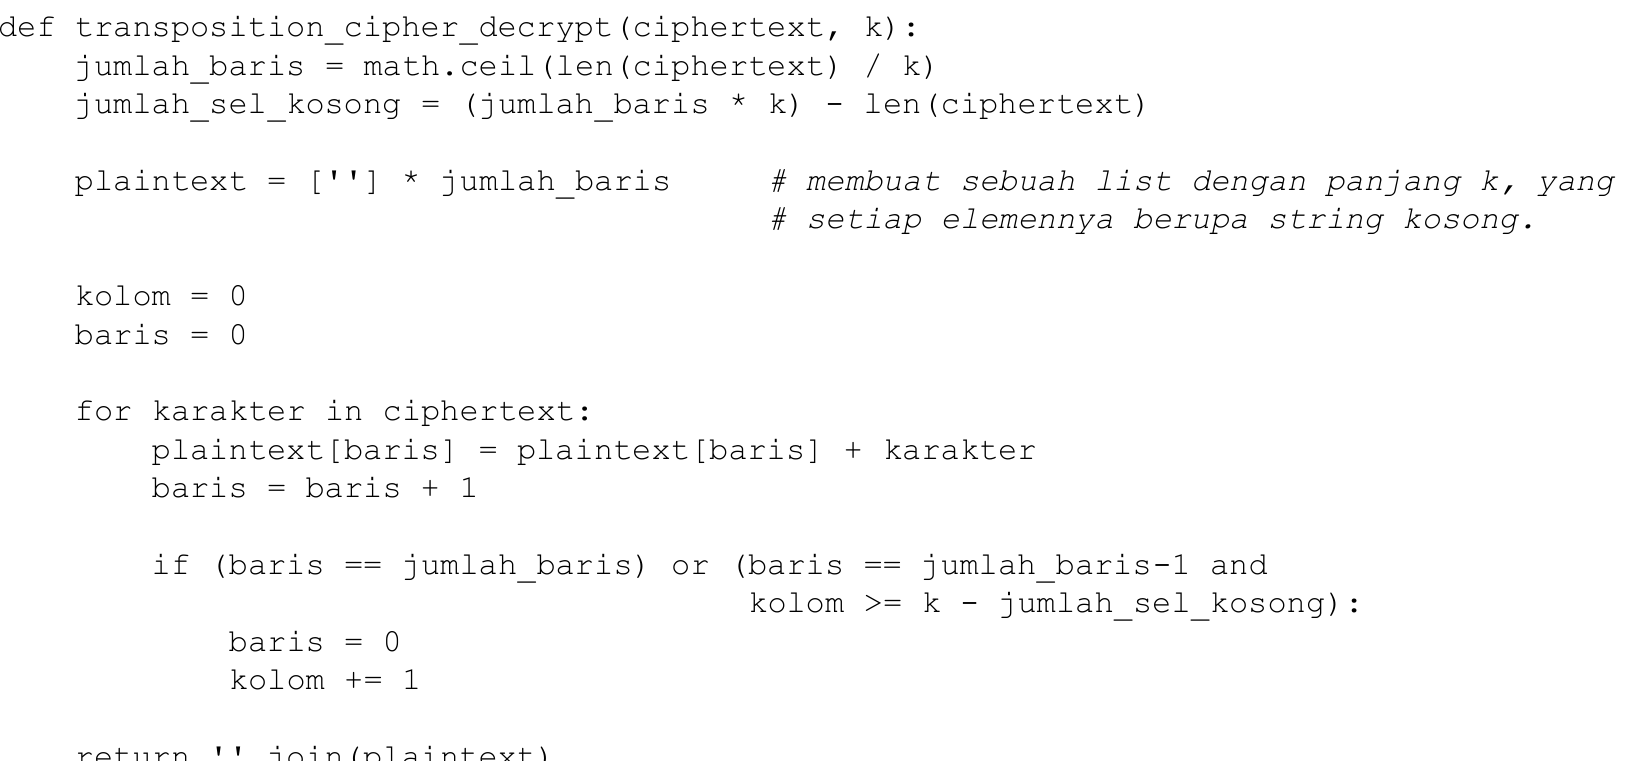
\includegraphics[width=178.29mm,height=209.38mm]{../../images/llm/page_037_img_01.png}%
\end{textblock*}

\end{document}
